\chapter{Software basato sul cloud}
\label{cap:cloud}

\begin{inbreve}
Il capitolo parte dai modelli di servizio del cloud (IaaS, PaaS, SaaS) e si concentra sul \emph{software as a service}:
vantaggi per chi lo offre e per chi lo usa, problemi di design. Poi confronta le due organizzazioni dei dati dei clienti,
multi-tenant e multi-instance. Infine raccoglie le decisioni architetturali di un prodotto cloud: database,
scalabilità e resilienza, struttura del software, piattaforma. Serve conoscere container e Docker
(capitolo~\ref{cap:container}); la struttura a servizi è sviluppata nel capitolo~\ref{cap:microservizi}.
\end{inbreve}

\section{Tutto come servizio}
\label{sec:cloud-aas}

Le risorse del cloud si offrono come servizio a tre livelli (\tabrif{tab:cloud-aas}).

\begin{definizione}[IaaS, PaaS, SaaS]
\begin{itemize}
  \item \textbf{IaaS} (\ingl{Infrastructure as a Service}) fornisce server, memoria di massa e rete (virtualizzati). Il provider
    gestisce tutta l'infrastruttura. Il cliente è responsabile di tutti gli altri aspetti della distribuzione (per
    esempio sistema operativo e applicazione). Esempi: EC2, S3.
  \item \textbf{PaaS} (\ingl{Platform as a Service}) fornisce un'intera piattaforma (VM, sistema operativo, servizi,
    SDK, \dots). Il provider gestisce infrastruttura, sistema operativo e software abilitante. Il cliente installa e
    gestisce l'applicazione. Esempi: Heroku, Azure, GAE.
  \item \textbf{SaaS} (\ingl{Software as a Service}) fornisce software su richiesta, accessibile con client leggeri (\ingl{thin client}) o
    API. Il provider gestisce infrastruttura, sistema operativo e applicazione. Il cliente non è responsabile di nulla.
    Esempio: salesforce.com.
\end{itemize}
\end{definizione}

\subsubsection{FaaS\aggiunta}
Il \termine{FaaS} (\ingl{Function as a Service}) è un quarto modello. Il cliente carica singole funzioni e il provider
le esegue solo quando arrivano le richieste. Il provider gestisce tutto il resto, comprese le risorse di calcolo, che
si pagano in base a quante volte la funzione viene eseguita.

\begin{table}[ht]
\centering
\small
\caption{Chi gestisce che cosa nei tre modelli di servizio\aggiunta}
\label{tab:cloud-aas}
\begin{tabular}{@{}lccc@{}}
\toprule
& IaaS & PaaS & SaaS \\
\midrule
Infrastruttura & provider & provider & provider \\
Sistema operativo & cliente & provider & provider \\
Software abilitante & cliente & provider & provider \\
Applicazione & cliente & cliente & provider \\
\bottomrule
\end{tabular}
\end{table}

\section{Software as a Service}
\label{sec:cloud-saas}

All'inizio i prodotti software erano installati sui computer dei clienti. Questo comportava tre problemi:
\begin{itemize}
  \item i clienti dovevano configurare il software;
  \item i clienti dovevano occuparsi degli aggiornamenti;
  \item l'azienda doveva mantenere versioni diverse del prodotto.
\end{itemize}

Con il \termine{SaaS} il prodotto è consegnato come servizio. I clienti non devono installare nulla, pagano un abbonamento
e accedono al prodotto da remoto.

\subsection{Benefici per chi offre il prodotto}

\begin{description}[leftmargin=0pt, style=unboxed]
  \item[Cash flow.] Flusso di cassa regolare: i clienti pagano un abbonamento periodico o in base all'uso.
  \item[Update management.] Il fornitore controlla gli aggiornamenti e i clienti li ricevono nello stesso momento. Non
    serve mantenere più versioni contemporaneamente, quindi i costi si riducono.
  \item[Continuous deployment.] Si può distribuire una nuova versione appena le modifiche sono fatte e collaudate.
  \item[Payment flexibility.] Diverse opzioni di pagamento attraggono più clienti. Per esempio le piccole aziende e i
    singoli evitano di pagare grandi costi iniziali.
  \item[Try before you buy.] Si può rendere disponibile presto una versione gratuita o a basso costo e raccogliere il riscontro dei clienti.
  \item[Data collection.] Si raccolgono facilmente dati sull'uso del prodotto e sui clienti.
\end{description}

\subsection{Pro e contro per i clienti}

\textbf{Vantaggi.} Accesso da mobile, laptop e desktop. Nessun costo iniziale per software o server. Aggiornamenti
immediati. Costi di gestione del software ridotti.

\textbf{Svantaggi.}
\begin{itemize}
  \item \emph{Conformità alle norme sulla privacy}: per esempio i paesi UE hanno leggi rigide sulla conservazione
    dei dati personali.
  \item \emph{Sicurezza}: i clienti possono non voler cedere il controllo dei dati a un fornitore esterno.
  \item \emph{Vincoli di rete}: possono limitare il tempo di risposta quando si trasferiscono molti dati.
  \item \emph{Scambio di dati}: può essere difficile se il cloud non offre un'API adatta.
  \item \emph{Perdita di controllo sugli aggiornamenti.}
  \item \emph{Service lock-in.}
\end{itemize}

\section{Questioni di design del SaaS}
\label{sec:cloud-design}

\begin{description}[leftmargin=0pt, style=unboxed]
  \item[Elaborazione locale o remota.] Alcune feature possono essere eseguite localmente. Vantaggi: meno traffico di rete
    e risposta più veloce. Svantaggio: maggior consumo di energia nei dispositivi a batteria.
  \item[Autenticazione.] Il prodotto può avere un proprio sistema di autenticazione oppure usare
    l'\emph{autenticazione federata}, con le credenziali individuali di servizi come Google o LinkedIn.
  \item[Information leakage.] Rischi di sicurezza dovuti a utenti multipli di organizzazioni diverse.
  \item[Gestione del database: multi-tenant o multi-instance.] Un unico repository, oppure copie separate del sistema e
    del database (\rif{sec:cloud-multitenant}, \rif{sec:cloud-multiistanza}).
\end{description}

\subsection{Autenticazione e fuga di informazioni\aggiunta}

Con un \emph{sistema di autenticazione proprio} il prodotto conserva le credenziali degli utenti e le verifica da
solo. Con l'\emph{autenticazione federata} l'utente si autentica presso un fornitore esterno (per esempio Google): il
prodotto riceve la conferma dell'identità e non conserva la password. Per un cliente aziendale questo permette di
usare le credenziali dell'azienda.

L'\emph{information leakage} è il rischio che i dati di un'organizzazione diventino visibili a utenti di un'altra.
Nasce quando utenti di organizzazioni diverse condividono lo stesso sistema, e si affronta con il controllo degli
accessi e la cifratura (\rif{sec:cloud-multitenant}).

\section{Sistemi multi-tenant}
\label{sec:cloud-multitenant}

\begin{definizione}[Sistema multi-tenant]
In un sistema \termine{multi-tenant} tutti gli utenti condividono un unico schema di database. Ogni voce del
database è etichettata con un identificatore del \termine{tenant} (cliente), così da offrire un ``isolamento logico''.
\end{definizione}

\begin{esempio}[Tabella multi-tenant]
Nella tabella \emph{Stock management} la colonna \texttt{Tenant} identifica il cliente.

\smallskip
\small
\begin{tabular}{@{}llllll@{}}
\toprule
Tenant & Key & Item & Stock & Supplier & Ordered \\
\midrule
T516 & 100 & Widg 1 & 27 & S13 & 2017/2/12 \\
T632 & 100 & Obj 1 & 5 & S13 & 2017/1/11 \\
T973 & 100 & Thing 1 & 241 & S13 & 2017/2/7 \\
T516 & 110 & Widg 2 & 14 & S13 & 2017/2/2 \\
T516 & 120 & Widg 3 & 17 & S13 & 2017/1/24 \\
T973 & 100 & Thing 2 & 132 & S26 & 2017/2/12 \\
\bottomrule
\end{tabular}
\end{esempio}

\begin{table}[ht]
\centering
\small
\caption{Vantaggi e svantaggi dei database multi-tenant.}
\label{tab:cloud-multitenant}
\begin{tabularx}{\linewidth}{>{\raggedright\arraybackslash}p{2.6cm}XX}
\toprule
& Vantaggi & Svantaggi \\
\midrule
Risorse / flessibilità & \emph{Resource utilization}: il provider SaaS controlla tutte le risorse usate dal
  software e può ottimizzarlo per usarle bene. & \emph{Inflexibility}: tutti i clienti usano lo stesso schema, con
  margini limitati di adattamento alle esigenze individuali (\rif{sec:cloud-schema}). \\
Sicurezza & \emph{Security}: i database multi-tenant devono essere progettati per la sicurezza, perché i dati di tutti i
  clienti stanno nello stesso database. Hanno quindi probabilmente meno vulnerabilità dei database standard. La gestione
  è semplificata: c'è una sola copia del software di database da correggere se si scopre una vulnerabilità. &
  \emph{Security}: esiste la possibilità teorica che i dati passino da un cliente all'altro. In pratica i casi sono
  pochissimi. Più grave, una violazione della sicurezza del database riguarda tutti i clienti. \\
Aggiornamenti / complessità & \emph{Update management}: è più facile aggiornare una sola istanza del software che molte.
  Gli aggiornamenti arrivano a tutti i clienti insieme, quindi tutti usano l'ultima versione. &
  \emph{Complexity}: i sistemi multi-tenant sono di solito più complessi di quelli multi-instance, perché devono gestire
  molti utenti. Aumenta quindi la probabilità di bug nel software del database. \\
\bottomrule
\end{tabularx}
\end{table}

\subsection{Personalizzazione}

Le aziende di dimensione media e grande raramente vogliono usare software multi-tenant generico. Spesso preferiscono
una versione personalizzata sulle proprie esigenze (\tabrif{tab:cloud-personalizzazioni}).

\begin{table}[ht]
\centering
\small
\caption{Possibili personalizzazioni di un SaaS.}
\label{tab:cloud-personalizzazioni}
\begin{tabularx}{\linewidth}{>{\raggedright\arraybackslash}p{3cm}X}
\toprule
Personalizzazione & Esigenza dell'azienda \\
\midrule
Authentication & Autenticare gli utenti con le credenziali aziendali invece di quelle impostate dal fornitore del software.
  L'autenticazione federata lo rende possibile. \\
Branding & Un'interfaccia con il marchio e l'identità visiva della propria organizzazione. \\
Business rules & Definire regole di business e flussi di lavoro propri, che si applicano ai propri dati. \\
Data schemas & Estendere il modello di dati standard del database per le proprie esigenze. \\
Access control & Definire un proprio modello di controllo degli accessi: quali dati possono usare utenti o gruppi
  specifici e quali operazioni sono consentite. \\
\bottomrule
\end{tabularx}
\end{table}

\subsubsection{Configurazione dell'interfaccia}
L'interfaccia si configura con i \termine{profili utente} (\figrif{fig:cloud-profili}). All'utente si chiede di
scegliere la sua organizzazione o di indicare l'indirizzo e-mail aziendale. Il prodotto usa le informazioni del
profilo per creare una versione personalizzata dell'interfaccia. Per esempio, il nome e il logo generici sono
sostituiti da quelli dell'azienda, oppure alcune voci di menu sono disattivate.

\begin{figure}[ht]
\centering
\begin{tikzpicture}[u/.style={draw, ellipse, font=\footnotesize, inner sep=2pt}, p/.style={font=\footnotesize}]
\node[draw, circle, minimum size=1.8cm, font=\small, align=center] (app) at (0,0) {SaaS\\application};
\node[draw, rounded corners=2pt, font=\footnotesize] (p1) at (-3.3,1.6) {Profile co1};
\node[draw, rounded corners=2pt, font=\footnotesize] (p2) at (0,2.1) {Profile co2};
\node[draw, rounded corners=2pt, font=\footnotesize] (p3) at (3.3,1.6) {Profile co3};
\foreach \p in {p1,p2,p3} \draw (app) -- (\p);
\node[u] at (-4.6,3.2) {co1 user}; \node[u] at (-2.4,3.2) {co1 user};
\node[u] at (-1.1,3.9) {co2 user}; \node[u] at (1.1,3.9) {co2 user};
\node[u] at (2.4,3.2) {co3 user}; \node[u] at (4.6,3.2) {co3 user};
\foreach \x/\y in {-4.6/3.2,-2.4/3.2} \draw (p1) -- (\x,\y-0.2);
\foreach \x/\y in {-1.1/3.9,1.1/3.9} \draw (p2) -- (\x,\y-0.2);
\foreach \x/\y in {2.4/3.2,4.6/3.2} \draw (p3) -- (\x,\y-0.2);
\end{tikzpicture}
\caption{Configurazione con i profili utente. Ogni utente appartiene a un'organizzazione (co1, co2, co3). L'applicazione
usa il profilo dell'organizzazione per adattare l'interfaccia.}
\label{fig:cloud-profili}
\end{figure}

\subsection{Adattare lo schema del database}
\label{sec:cloud-schema}

Gli utenti aziendali possono voler estendere lo schema del database per le proprie esigenze. Ci sono due soluzioni.

\begin{description}[leftmargin=0pt, style=unboxed]
  \item[Soluzione I: colonne extra.] Si aggiunge a ogni tabella un certo numero di campi extra (\texttt{Ext 1},
    \texttt{Ext 2}, \texttt{Ext 3}, \dots) che i clienti usano come vogliono. Problemi:
    \begin{itemize}
      \item è difficile sapere quante colonne extra inserire: troppo poche non bastano, troppe sprecano spazio;
      \item clienti diversi richiederanno probabilmente tipi di colonne diversi.
    \end{itemize}
  \item[Soluzione II: extension table.] Si aggiunge a ogni tabella un campo che identifica una \emph{extension
    table} separata, e i clienti creano queste tabelle in base alle proprie necessità. Problema: maggiore
    complessità.
\end{description}

\begin{esempio}[Extension table]
Nella tabella principale, per ogni riga c'è un identificatore di estensione (colonna \texttt{Ext 1}). Una tabella
dei \emph{nomi dei campi} dice, per ogni tenant, quali campi aggiuntivi ha. Una tabella dei \emph{valori} contiene i
valori per ogni record.

\smallskip
\small
\begin{minipage}[t]{0.46\linewidth}
\textbf{Tabella principale} (estratto)\par\smallskip
\begin{tabular}{@{}lllr@{\qquad}l@{}}
\toprule
Tenant & ID & Item & Stock & Ext 1 \\
\midrule
T516 & 100 & Widg 1 & 27 & E123 \\
T632 & 100 & Obj 1 & 5 & E200 \\
T973 & 100 & Thing 1 & 241 & E346 \\
\bottomrule
\end{tabular}
\end{minipage}\hfill
\begin{minipage}[t]{0.5\linewidth}
\textbf{Nomi dei campi}\par\smallskip
\begin{tabular}{@{}lll@{}}
\toprule
Tenant & Nome & Tipo \\
\midrule
T516 & Location & String \\
T516 & Weight & Integer \\
T516 & Fragile & Bool \\
T632 & Delivered & Date \\
T632 & Place & String \\
T973 & Delivered & Date \\
\bottomrule
\end{tabular}
\end{minipage}

\medskip
\begin{minipage}[t]{0.6\linewidth}
\textbf{Valori dei campi}\par\smallskip
\begin{tabular}{@{}lll@{}}
\toprule
Record & Tenant & Valore \\
\midrule
E123 & T516 & `A17/S6' \\
E123 & T516 & `4' \\
E123 & T516 & `False' \\
E200 & T632 & `2017/1/15' \\
E200 & T632 & `Dublin' \\
E346 & T973 & `2017/2/10' \\
\bottomrule
\end{tabular}
\end{minipage}

\smallskip
Così i campi estesi per T516, voce 100, sono \emph{Location}, \emph{Weight} e \emph{Fragile}, con valori
`A17/S6', `4' e `False'. Quelli per T632, voce 100, sono \emph{Delivered} e \emph{Place}, con valori `2017/1/15' e
`Dublin'.
\end{esempio}

\subsection{Sicurezza}

La sicurezza è la preoccupazione principale dei clienti aziendali dei database multi-tenant. I dati di tutti i clienti
stanno nello stesso database: un bug del software o un attacco potrebbero esporre i dati di alcuni o di tutti i clienti
agli altri. Servono due misure.

\begin{itemize}
  \item \textbf{Multilevel access control}: l'accesso ai dati va controllato a livello di organizzazione e a livello di
    singolo utente. Il controllo a livello di organizzazione garantisce che ogni operazione sul database riguardi solo i
    dati di quell'organizzazione. I singoli utenti hanno inoltre i propri permessi di accesso.
  \item \textbf{Encryption}: rassicura i clienti aziendali che i loro dati non possano essere visti da persone di altre
    aziende in caso di malfunzionamento. I dati cifrati si decifrano solo con la chiave appropriata. Cifratura e
    decifratura sono operazioni onerose, quindi di solito si cifrano solo i dati sensibili.
\end{itemize}

\section{Sistemi multi-instance}
\label{sec:cloud-multiistanza}

\begin{definizione}[Sistema multi-instance]
In un sistema \termine{multi-instance} ogni cliente ha un proprio sistema, adattato alle sue esigenze, con il proprio
database e i propri controlli di sicurezza.
\end{definizione}

Rispetto al multi-tenant è concettualmente più semplice. Evita anche i problemi di sicurezza come la fuga di dati tra
organizzazioni. Esistono due tipi:

\begin{itemize}
  \item \textbf{basati su VM}: l'istanza software e il database di ogni cliente girano in una VM propria. Tutti gli
    utenti dello stesso cliente possono accedere al database di sistema condiviso;
  \item \textbf{basati su container}: ogni utente ha una versione isolata del software e del database, che gira in un
    insieme di container. È adatto soprattutto ai prodotti in cui gli utenti lavorano per lo più in modo indipendente,
    con poca condivisione dei dati (per esempio per utenti individuali).
\end{itemize}

I container possono anche girare dentro una VM: un'azienda può avere un sistema basato su VM e far girare sopra di
esso i container per i singoli utenti.

\begin{table}[ht]
\centering
\small
\caption{Pro e contro dei database multi-instance.}
\label{tab:cloud-multiistanza}
\begin{tabularx}{\linewidth}{>{\raggedright\arraybackslash}p{2.6cm}XX}
\toprule
& Vantaggi & Svantaggi \\
\midrule
Flessibilità / costo & \emph{Flexibility}: ogni istanza può essere adattata alle esigenze del cliente, che può
  usare schemi di database completamente diversi. È semplice trasferire dati da un database del cliente a quello del
  prodotto. & \emph{Cost}: costa di più, per l'affitto di molte VM nel cloud e per la gestione di più sistemi. A
  causa del lento avvio delle VM, può servire tenerle affittate e in funzione di continuo, anche con poca domanda. \\
Sicurezza & \emph{Security}: ogni cliente ha il proprio database, quindi non c'è possibilità di fuga di dati da un
  cliente a un altro. & \\
Scalabilità & \emph{Scalability}: le istanze si possono scalare in base alle necessità del singolo cliente. Per esempio
  alcuni clienti possono richiedere server più potenti. & \\
Resilienza / aggiornamenti & \emph{Resilience}: un guasto del software riguarderà probabilmente un solo cliente. Gli
  altri possono lavorare normalmente. & \emph{Update management}: molte istanze vanno aggiornate, quindi gli aggiornamenti
  sono più complessi, soprattutto se le istanze sono state adattate ai singoli clienti. \\
\bottomrule
\end{tabularx}
\end{table}

\section{Decisioni architetturali}
\label{sec:cloud-decisioni}

Un prodotto cloud richiede quattro decisioni architetturali (\figrif{fig:cloud-decisioni}).

\begin{figure}[ht]
\centering
\begin{tikzpicture}[q/.style={draw, rounded corners=6pt, minimum width=4cm, align=center, font=\small, inner sep=5pt}]
\node[q] (d) at (-4.7,2.2) {Il software deve usare un\\database multi-tenant\\o multi-instance?};
\node[q] (s) at (0,2.2) {Quali requisiti di\\scalabilità e resilienza\\ha il software?};
\node[q] (t) at (4.7,2.2) {Il software deve avere\\struttura monolitica\\o orientata ai servizi?};
\node[q] (c) at (0,0) {Quale piattaforma cloud\\usare per sviluppo\\e consegna?};
\draw[freccia] (d.south) |- (c.west);
\draw[freccia] (s) -- (c);
\draw[freccia] (t.south) |- (c.east);
\node[font=\footnotesize\sffamily, above=1pt of d] {Database organization};
\node[font=\footnotesize\sffamily, above=1pt of s] {Scalability and resilience};
\node[font=\footnotesize\sffamily, above=1pt of t] {Software structure};
\end{tikzpicture}
\caption{Le quattro decisioni architetturali. Le prime tre (database, scalabilità e resilienza, struttura del software)
condizionano la scelta della piattaforma cloud.}
\label{fig:cloud-decisioni}
\end{figure}

\subsection{Organizzazione del database}
\label{sec:cloud-db}

Un database dei clienti in un sistema cloud si può fornire in tre modi:
\begin{enumerate}
  \item come sistema \emph{multi-tenant}, condiviso da tutti i clienti del prodotto, ospitato nel cloud su server grandi e
    potenti;
  \item come sistema \emph{multi-instance}, con il database di ogni cliente in una VM propria;
  \item come sistema \emph{multi-instance}, con ogni database in un container proprio. Il database del cliente può
    essere distribuito su più container.
\end{enumerate}

La scelta dipende da cinque fattori (\tabrif{tab:cloud-fattori-db}).

\begin{table}[ht]
\centering
\small
\caption{Fattori che guidano la scelta del tipo di database.}
\label{tab:cloud-fattori-db}
\begin{tabularx}{\linewidth}{>{\raggedright\arraybackslash}p{3.2cm}X}
\toprule
Fattore & Domande chiave \\
\midrule
Target customers & I clienti richiedono schemi di database e personalizzazione diversi? Hanno preoccupazioni di
  sicurezza sulla condivisione del database? Se sì, usare un database multi-instance. \\
Transaction requirements & È critico che il prodotto supporti transazioni ACID (\rif{sec:micro-dati}), in cui i dati sono
  sempre garantiti coerenti? Se sì, usare un database multi-tenant o un database multi-instance basato su VM. \\
Database size and connectivity & Quanto è grande il database tipico dei clienti? Quante relazioni ci sono tra le voci?
  Un modello multi-tenant è di solito il migliore per database molto grandi, perché si può concentrare l'impegno
  sull'ottimizzazione delle prestazioni. \\
Database interoperability & I clienti vorranno trasferire informazioni da database esistenti? Quali sono le
  differenze tra gli schemi? Quale supporto software si aspettano per il trasferimento? Se i clienti hanno molti
  schemi diversi, usare un database multi-instance. \\
System structure & Il sistema usa un'architettura orientata ai servizi? I database dei clienti si possono dividere in
  database di servizi individuali? Se sì, usare database multi-instance containerizzati. \\
\bottomrule
\end{tabularx}
\end{table}

Clienti diversi hanno aspettative diverse. Tre esempi:
\begin{itemize}
  \item consumatori o piccole aziende non si aspettano personalizzazione e marchio, un sistema di autenticazione
    locale o permessi individuali diversi: basta un database multi-tenant con un solo schema;
  \item le grandi aziende vogliono più spesso un database adattato alle proprie esigenze: è possibile in parte con un
    sistema multi-tenant, più facile con un database multi-instance;
  \item se il database deve essere sempre coerente (per esempio in finanza) serve un sistema transazionale: un database
    multi-tenant oppure un database per cliente su VM (con tutti gli utenti del cliente che condividono il
    database basato su VM).
\end{itemize}

\subsection{Scalabilità e resilienza}
\label{sec:cloud-scal}

\begin{definizione}[Scalability]
La \termine{scalabilità} è la capacità di adattarsi automaticamente alle variazioni del carico. Si ottiene
\emph{aggiungendo nuovi server virtuali} (\ingl{scaling out}) oppure \emph{aumentando la potenza di un server} del sistema
(\ingl{scaling up}) in risposta al carico crescente.
\end{definizione}

\begin{esempio}[Scaling out e scaling up\aggiunta]
Ogni istanza di un servizio regge 100 richieste al secondo. Arrivano 450 richieste al secondo. Con lo
\emph{scaling out} si avviano $\lceil 450/100 \rceil = 5$ istanze e un load balancer le ripartisce. Con lo
\emph{scaling up} si sostituisce il server con uno circa 4,5 volte più potente. Se il carico scende a 150 richieste al
secondo, lo scaling out toglie 3 istanze (ne bastano 2) e si paga solo ciò che serve. Lo scaling up ha un limite: non
esiste un server potente quanto si vuole.
\end{esempio}

Nei sistemi basati sul cloud è tipico lo scaling out. Il prodotto deve essere organizzato in modo che i singoli
componenti software possano essere replicati ed eseguiti in parallelo. Meccanismi di \emph{load balancing} inviano le
richieste a istanze diverse dei componenti (per esempio con PaaS).

\begin{definizione}[Resilience]
La \termine{resilienza} è la capacità di continuare a fornire i servizi critici in caso di guasto del sistema o di uso
malevolo.
\end{definizione}

Nella soluzione \termine{hot standby} (\figrif{fig:cloud-hotstandby}):
\begin{itemize}
  \item repliche del software e dei dati sono mantenute in luoghi diversi;
  \item gli aggiornamenti del database sono replicati (\emph{mirrored});
  \item un \emph{system monitor} controlla di continuo lo stato del sistema.
\end{itemize}
Un'alternativa più economica è il \termine{cool standby}: i dati sono ripristinati da un backup e il sistema non è
disponibile finché il ripristino non è completato.

\begin{figure}[ht]
\centering
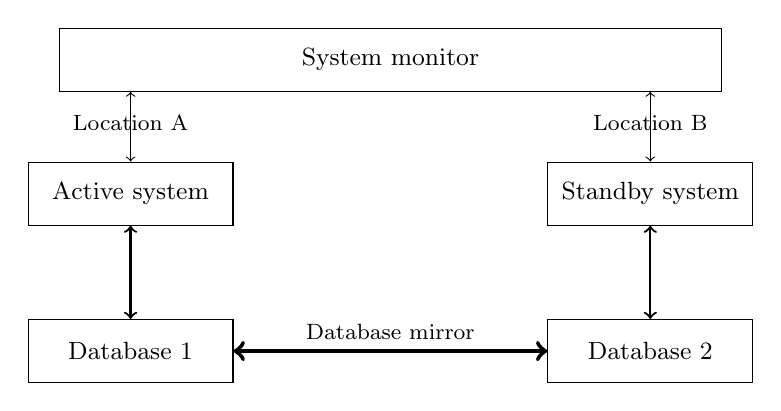
\begin{tikzpicture}[b/.style={draw, minimum width=2.6cm, minimum height=0.8cm, font=\small, align=center}]
\node[b, minimum width=8.4cm] (m) at (3.3,3.4) {System monitor};
\node[font=\footnotesize] at (0,2.6) {Location A};
\node[font=\footnotesize] at (6.6,2.6) {Location B};
\node[b] (a) at (0,1.7) {Active system};
\node[b] (s) at (6.6,1.7) {Standby system};
\node[b] (d1) at (0,-0.3) {Database 1};
\node[b] (d2) at (6.6,-0.3) {Database 2};
\draw[<->] (m.south -| a) -- (a);
\draw[<->] (m.south -| s) -- (s);
\draw[<->, thick] (a) -- (d1);
\draw[<->, thick] (s) -- (d2);
\draw[<->, ultra thick] (d1) -- node[above, font=\footnotesize] {Database mirror} (d2);
\end{tikzpicture}
\caption{Hot standby. Un sistema attivo nella sede A e un sistema in attesa nella sede B, ciascuno con il proprio
database. Il database è replicato in modo continuo tra le sedi. Il system monitor controlla entrambi i sistemi.}
\label{fig:cloud-hotstandby}
\end{figure}

\subsection{Struttura del software}
\label{sec:cloud-struttura}

Le due strutture sono la \emph{monolitica} (un unico blocco software) e quella a \emph{servizi stateless a grana
fine} (\ingl{fine-grain}). Un servizio \emph{stateless} non mantiene stato interno (\rif{sec:micro-servizi}).
I servizi sono indipendenti e si possono replicare, distribuire e migrare. Sono particolarmente adatti al software per il cloud, con servizi
distribuiti nei container.

L'approccio monolitico è spesso usato per costruire un prototipo. Quando parti diverse vanno aggiornate in momenti
diversi, e solo alcune parti devono scalare, si usano i \emph{microservizi} (capitolo~\ref{cap:microservizi}).

\subsection{Piattaforma cloud}
\label{sec:cloud-piattaforma}

La scelta della piattaforma cloud ha aspetti tecnici e di business.

\textbf{Questioni tecniche.}
\begin{itemize}
  \item carico atteso e sua prevedibilità;
  \item resilienza;
  \item servizi cloud supportati;
  \item privacy e protezione dei dati. Per esempio i paesi UE hanno requisiti rigidi sulla protezione dei dati e
    su dove sono conservati: serve un provider che dia garanzie sui luoghi di conservazione.
\end{itemize}

\textbf{Questioni di business.}
\begin{itemize}
  \item \emph{costo}: compromesso tra costi diretti e indiretti (per esempio la gestione del cloud);
  \item \emph{esperienza degli sviluppatori};
  \item \emph{clienti}: il prodotto può dover interagire con altro software usato dai clienti, e alcune
    aziende preferiscono fornitori di fiducia;
  \item \emph{service-level agreements}: la qualità del servizio (QoS) è davvero ``garantita''?
  \item \emph{portabilità e migrazione}: conviene preparare un ``piano di uscita'' (\ingl{exit plan}) per ridurre il
    vendor lock-in (questione sia tecnica sia di business).
\end{itemize}

\begin{puntichiave}
\begin{itemize}
  \item IaaS: il cliente gestisce sistema operativo e applicazione. PaaS: il cliente gestisce solo l'applicazione.
    SaaS: il cliente non gestisce nulla.
  \item SaaS: cash flow regolare, aggiornamenti per tutti insieme, continuous deployment. Per i clienti: nessun costo
    iniziale ma rischi di sicurezza, privacy, lock-in.
  \item Multi-tenant: un solo schema condiviso, dati etichettati con il tenant. Personalizzazione con profili, colonne
    extra o extension table. Sicurezza: controllo degli accessi a più livelli e cifratura.
  \item Multi-instance: sistema e database per ogni cliente, su VM o su container. Più flessibile e sicuro, più costoso.
  \item La scelta del database dipende da clienti, transazioni, dimensioni, interoperabilità e struttura del sistema.
  \item Scalabilità: scaling out (più server virtuali) o scaling up. Resilienza: hot standby o cool standby.
  \item Monolite per il prototipo; servizi stateless a grana fine (microservizi) per scalare e aggiornare parti
    diverse.
\end{itemize}
\end{puntichiave}

\begin{domande}
\begin{enumerate}
  \item Che differenza c'è tra IaaS, PaaS e SaaS e chi gestisce che cosa?
  \item Quali sono i benefici del SaaS per il fornitore e per il cliente? Quali i rischi?
  \item Che cos'è un sistema multi-tenant e come si garantisce l'isolamento logico?
  \item Come si adatta lo schema di un database multi-tenant? Confrontare le due soluzioni.
  \item Quali misure di sicurezza servono nei database multi-tenant?
  \item Che cosa sono i sistemi multi-instance e quali tipi esistono? Quali sono pro e contro?
  \item Quali fattori guidano la scelta tra database multi-tenant e multi-instance?
  \item Che cosa sono scaling out e scaling up? Che differenza c'è tra hot e cool standby?
  \item Quali questioni tecniche e di business guidano la scelta della piattaforma cloud?
\end{enumerate}
\end{domande}
